\chapter{Evaluation}
\label{ch:Evaluation}
In this chapter we evaluate the contributions of this thesis and the general state of the project. On that account we first examine the changes to the UI, the Source Code Previews and performance improvements. We then verify the most important features of CRI by checking a set of specifications for each test application and discuss the result.

All performance measurements and tests in this chapter were performed with Chrome Version 64.0.3282.140 (Offizieller Build) (64-Bit), WebStorm 2017 3.4 and Windows 10 Home 64 bit version 1709 build 16299.192. The used device has 8GB RAM, Intel i7 7500 2.7GHz 4CPUs Processor with integrated Intel(R) HD Graphics 620. Each test application was hosted on the integrated Web server of WebStorm on the local machine. No other applications were running, but background processes and services as well as other unpredictable factors have to be taken into account that may have influenced the results of the performance measurements.

\section{Evaluation of Improvements}
This section examines the improvements introduced by this thesis and their implementations. We inspect the changes made to the UI as well as the Source Code Tooltips and their applicability in the test applications. At last, we examine the performance improvements introduced by this thesis in comparison with the previous version of CRI.  

	\subsection{Changes to the User Interface}
	Most of the changes to the User Interface are, by their nature, hard to evaluate in regards to their usability improvement. The experienced usability of a UI can be highly subjective \cite, the easiest way to achieve consistent evaluation results is therefore by collecting and analyzing empirical data, for example through Click stream analysis \cite{Clickstream}. Since CRI is not yet used in active production systems by a large user base, a User Study would be the usual approach. Unfortunately this is outside the scope of this thesis. However, some changes are verified as improvements. For example, the text per node in the Dependency Graph was reduced without loosing any information can be seen as a general improvement of usability, because the change did not affect any other part of the UI and removed obsolete text. Another change that can be objectively categorized as an improvement is that parts of the UI which are not necessary to examine the Dependency Graph can now be hidden. Although it has to be noted that this change added a new UI element - the \emph{hide} button - which could potentially introduces new usability issues. Highlighting of the currently updated edge in addition to nodes also provides additional information for the user, to help track down differences between steps that were not as easily detectable before, without affecting other aspects of the UI.

	\subsection{Inspecting Source Code Tooltips}
	The Source Code Tooltips that connect nodes in the Dependency Graph with the JS code they originate from are created whenever the user hovers over a node and presses the CTRL key. Due to their on-demand nature, their performance impact on the time critical computations of CRI like the recording process can be neglected. The original JS files are stored in a variable in a Content script of CRI that are queried for the lines corresponding to a node if requested. Storing a copy of the whole JS file in addition to the instrumented version however should not exceed the Memory (RAM) of any modern computer that runs Google Chrome. We will examine the robustness of this feature in regards to its accuracy in a later section as part of the test application evaluation. To investigate and verify the usefulness of Source Code Tooltips we examined each test application and calculated the percentage of nodes that gain additional context through this feature. As a \emph{named} node already has some form of context that helps the user to identify it and its dependents, we counted \emph{named} nodes separately. For the exact circumstances and inputs used for each test application see section \ref{sec:EvalTests}. Over all test applications there were 586 nodes. Of these, 440 nodes had a Source Code Tooltip which equals to approximately 75\% of all nodes. Only 199, approximately 33.9\% of all nodes are \emph{named}. This means that the introduction of Source Code Tooltips provided additional means to identify a node to the user for 35.1\% of the total number of nodes. The remaining 146 nodes that can not yet be linked to specific positions in the source code in part consist of nodes that can be easily interpreted by examining the nodes that depend on them. For example in the test application \emph{RXJS canvas-painting}
	the node with Id 6 is a FromEventObservable created by "Rx.Observable.fromEvent(colorchar,"click")" and is not yet detected by the Jalangi analysis.

	\subsection{Scrutinizing performance with rapidly updated Observables}
	\label{sec:PerformanceEvaluation}
	In this section we evaluate the performance improvements resulting from the reworked graph history and the less frequent UI rendering in detail. To this purpose we developed a new test application for RxJS which is used as a simple benchmark on how well a CRI, and in the last part of this section RxFiddle, cope with a simple rapidly updating observable. The application uses an Interval Observable to generate one update every five milliseconds over a period of five seconds. In listing \ref{lst:performanceTestExtract} the Observable responsible for the updates is shown. The full source code with the termination after five seconds can be viewed in the appendix \ref{ch:Appendix}. %TODO okay to use that sentence?
	
	\begin{lstlisting}[language=JavaScript, caption={Example of RxJS code.},label={lst:performanceTestExtract}]
	var intervalObservable = Rx.Observable.interval(5)
	.timestamp()
	.bufferCount(2, 1)
	.map(function (w) {
	return w[1].timestamp - w[0].timestamp;
	})
	.share();	
	\end{lstlisting}

	To exclude the initial setup of CRI from the gathered performance data we create a Reactive Breakpoint for the \emph{nodeCreated} event of node one ("nodeCreated[1]"), ran the application until it paused at the Reactive Breakpoint, started the performance recording and then continued execution. To record a CPU profile that includes the time spent per function we used the Chrome-JavaScript Profiler. To inspect the memory usage we used the Memory tab of Chrome DevTools. The duration of the recordings vary from the actual time the execution of the test application took and its recording took, because they were started and ended manually. 
	
	\textbf{CPU Profile}
	\begin{figure}[!h]
	\centering
	\subfloat[Chrome Reactive Inspector version 2.0]{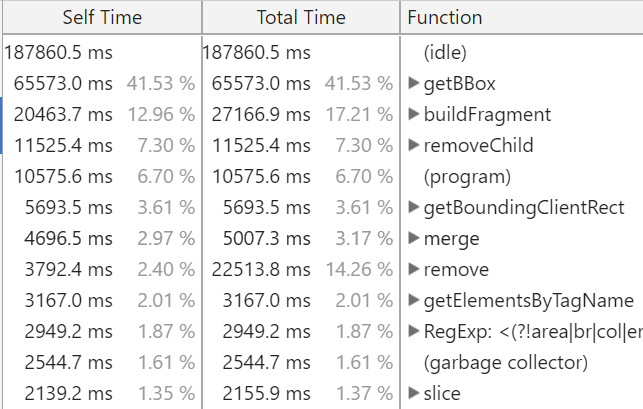
\includegraphics[width=0.4\textwidth]{gfx/CPU_CRI2.png}\label{fig:CPUCRI2}}
	\hfill
	\subfloat[Chrome Reactive Inspector version 3.0]{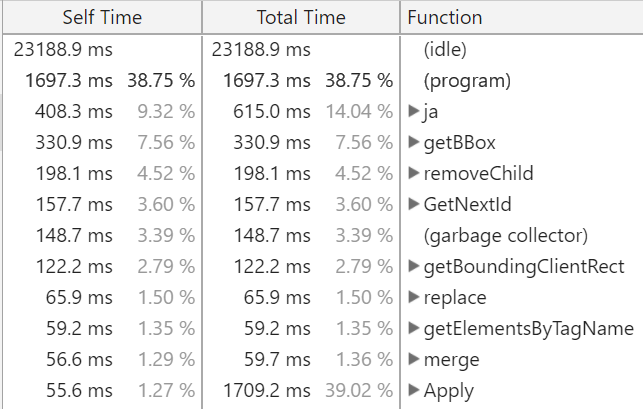
\includegraphics[width=0.4\textwidth]{gfx/CPU_CRI3.png}\label{fig:CPUCRI3}}
	\caption{CPU Profiles recorded by Google Chrome JavaScript Profiler.}
	\end{figure}
	
	The label "(program)" in the recording entitles native code execution of Chrome. The measured execution time for this label is far less accurate than any other measurement, because the individual composition is unclear and can solely increase by stopping the recording at a later point in time due to the limitations of the recording tool.
	
	For CRI2 the execution of PerformanceTest took approximately 154.0 seconds with an overall recording interval of 187.9 seconds. To differentiate between execution time and recording time we selected an area with significantly higher CPU load that should correspond reasonably well to the actual execution time. The largest percentage of \emph{Self Time} (the time spent executing code directly in the function) spent in a single function directly correspond to excessive UI updates - which happen at least once per created step since the slider is updated and triggers the rendering of a new Dependency Graph for that step. \emph{getBB} (getBoundingBox) calculates the size of nodes in the graph, whereas  \emph{buildFragment}'s impact stems form the \emph{domManip} function of jQuery.
	For CRI3 the execution took approximately 5.5 seconds with an overall recording interval of 23.2 seconds. It is visible that still a sizable amount of time is spent inside UI related computations especially \emph{getBB}. The most time of execution not related to Chromes native code is spent inside the \emph{ja} function of jQuery that can not easily be tracked down to CRI code. Overall the most time is spent inside Chromes native code, but as described earlier this can have numerous reasons. Due to the nature of changes from CRI2 to CRI3 we are however able to account at least part of that execution time to storage operations using the Chrome Storage API. 
	As CRI3 was approximately 28 times faster than CRI2, the performance improvements regarding rapid updates implemented by this thesis were effective. It is however worth noting, that CRI2 is barely able to handle this test without crashing - the UI becomes temporarily unresponsive. This probably increases the performance differences between the two versions of CRI more than it is for a test both CRI versions handle well (without the UI becoming temporarily unresponsive). We chose to keep the test as-is to underline the impact of \emph{request buildup} and load exceeding the extension's capacity. 
	As of now CRI3 also has a fixed capacity of updates it is able to handle without crashing, but it is much higher than CRI2's mostly due to the throttling of rendering operations. Basic tools to detect and react to an application exceeding that capacity are already in place for CRI3 and could be easily extended to automatically detect if rendering computations accumulate beyond its limit and increase or decrease the throttle interval for UI updates on demand. Since all steps are recorded even if the rendering is not able to keep up, increasing the throttle time to keep the extension from crashing is a viable approach. The user is then able to pause the recording anytime and examine the steps in details whereas a crash will render CRI useless to the user.
	
	\textbf{Memory Profiling}
	To reveal the impact of a large History on Memory consumption we executed the PerformanceTest with a limit of 250ms for both versions of CRI in addition to the execution we used for CPU profiling with a limit of five seconds.
	
	\begin{figure}[!h]
		\centering
		\subfloat[CRI2 - 5s duration]{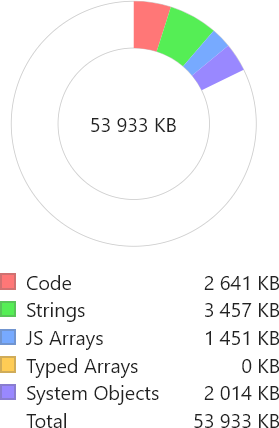
\includegraphics[width=0.4\textwidth]{gfx/RAM_CRI2.png}\label{fig:RAM2}}
		\hfill
		\subfloat[CRI3 - 5s duration]{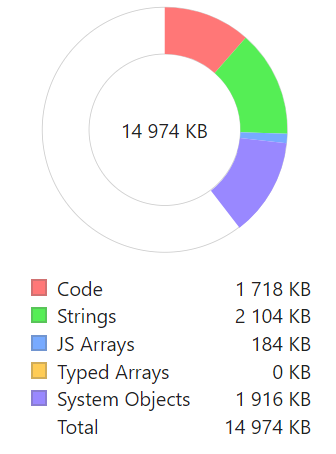
\includegraphics[width=0.4\textwidth]{gfx/RAM_CRI3.png}\label{fig:RAM3}}
		\subfloat[CRI2 - 250ms duration]{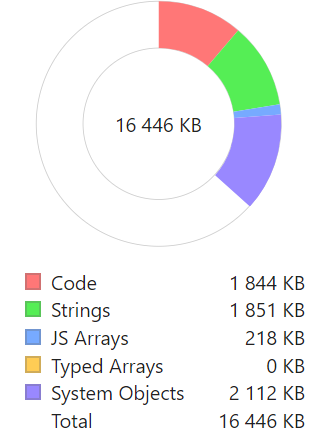
\includegraphics[width=0.4\textwidth]{gfx/RAM_CRI2_250ms.png}\label{fig:RAM2Short}}
		\subfloat[CRI3 - 250ms duration]{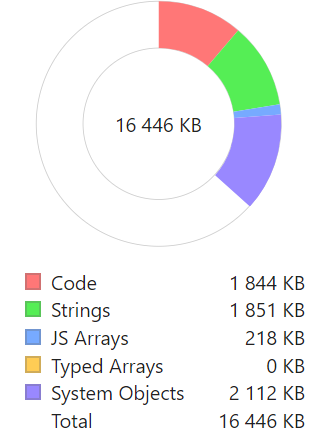
\includegraphics[width=0.4\textwidth]{gfx/RAM_CRI2_250ms.png}\label{fig:RAM3Short}}
		\caption{Memory Profiles recorded by Google Chrome Memory DevTool}
	\end{figure}
	
	For the test execution with the full duration (figure -ref-) CRI2 used 52.7MB in total while CRI3 used only 14.6MB. The most notable difference in a specific category is the size of the Memory used by JS arrays which includes the stored Dependency Graph. In the test with reduced execution time (250ms), CRI2 used approximately 16.1MB of Memory while CRI3 used 12.6MB of Memory. Both versions of CRI have a similar Memory consumption for the test with reduced execution time, although CRI2 shows the Dependency Graph with a noticeable delay (still less than 5s). Since CRI3's History implements a stream like approach through paging, the memory usage once the size of a single \emph{page} is exceeded is fairly constant and does not increase with the number of steps. As CRI2's History does not support paging the memory usage increases approximately proportional to the number of steps in the History. However since modern computers have usually more than 1GB of Memory, even the higher Memory consumption of CRI2 does not have any influence detectable by the user. We made no distinction of CRI3 with Delta Encoding and Paging; and CRI3 just with Paging, because this examination shows that the Memory usage is far to low to  imposes any limitation on the overall performance of CRI, even for CRI2.
	
	As there were no significant changes to the recording process of RxJS and BaconJS in CRI, we did not execute separate performance measurements for CRI2 and CRI3 using a test application with BaconJS.
	
	\textbf{Comparison to RxFiddle}
	We also examined the performance of RxFiddle with the used test application and compared it to CRI3 to qualify the discussion in section \ref{sec:RxFiddle} on its performance with rapidly updated Observables.
	Although RxFiddle does not have performance issues (exceeding a delay of one second when hovering over a node before the tooltip is shown) for approximately one thousand updates on Chrome, if executed with Firefox (57.0.4 (64-bit)) the browser becomes unresponsive for a few seconds. The overall Memory consumption of RxFiddle during the test was 52.5MB and the execution took approximately 5.5 seconds - similar to CRI3. As mentioned earlier the Memory consumption is not a limiting factor for the overall performance. CRI generates approximately 2700 steps during the test execution while RxFiddle generates approximately one thousand values for each Operator in the chain of \emph{intervalObservable}. Examining these results any further does not provide additional insight since the tools are bases on completely different technologies. RxFiddle uses TypeScript and runs as a Web page while CRI does not use TypeScript, any form of bundling or minifying and runs as a Chrome extension.
	
\section{Reviewing the Test Applications}
\label{sec:EvalTests}
To establish the current state of the most important features of CRI we compiled a set of specifications that we validated for each of the test applications. They were also designed to provide a baseline for the robustness of the current CRI implementation. Note that we also included specifications targeting features not introduced by this thesis as a means of manual regression testing for the most important aspects of CRI. Since most of these specifications can not be tested for each node, step and/or case in reasonable time, we specified the exact tests that were performed in order to approximate the results. These test probes should provide a reasonably precise evaluation and, in contrast to some of the specifications, are easy to reproduce in order to verify our results.

\textbf{Specifications}
\begin{itemize}
	\item[Spec1] The dependency graph is shown and all observables that are assigned to a named variable are displayed distinctively. (Test: Up to the first five named observables in the code are all displayed with an orange background.)
	\item[Spec2] The history of the dependency graph can be navigated. It is possible to navigate to the previous, succeeding or a random step in the history. (Test: Jump to the median step; click next five times; click previous five times.)
	\item[Spec3] For each node, no space is occupied by fields that hold no value in neither the node itself nor it's tooltip.
	\item[Spec4] The ids of the nodes start at one and are continuous. If the test application is started again with the exact same inputs, each node has the same id as in the last execution.
	\item[Spec5] The Source Code Tooltips show and highlight the corresponding lines of code for each node that has one. (Test: If possible, choose two nodes, one that corresponds to the middle of a chain of reactive function calls and one that corresponds to the end of a chain of reactive function calls. For both nodes check if the highlighting is correct.)
	\item[Spec6] The node or edge that was updated in a step is highlighted. (Test: Check this behavior for the first ten steps in the history.)
	\item[Spec7] The history queries can be used to search for a specific event in the history. (Test: Queries for \emph{evaluationYielded} and \emph{nodeUpdated} find the corresponding steps for the first named node.)
	\item[Spec8] The graph can be searched, the matching node(s) is/are highlighted and if the search is reseted the original coloring is restored. (Test: Search for the dependencies and dependents of the first named node and then reset the search.)
	\item[Spec9] Reactive breakpoints can be used to pause the debugger when a specific event occurs. (Test: \emph{a)} A breakpoint set for the first node created will break at step one. \emph{b)} A breakpoint for the first node updated will break before the value is updated in the original observable. Note: The value will be already updated in the CRI UI.)
\end{itemize}

We excluded some of the test applications that were used in the prior works targeting CRI from this evaluation, because they no longer work due to outside influences or did not provide any additional value. The results of this evaluation are visible in tables \ref{tab:RxJSa}, \ref{tab:RxJSb} and \ref{tab:BaconJS}. For the following statistics we interpreted \emph{ambiguity} labeled with \emph{Am} as if the check failed, because CRI is not able to handle ambiguity between nodes with the same name yet. \emph{N.A.} means that the check was not applicable e.g. because there were no \emph{Named} nodes in the Dependency Graph and the check is dependent on \emph{Named} nodes. We therefore treated \emph{N.A.} as a success. Due to specification number 9 having two parts that can fail or succeed individually we treated their result separately in the following statistic. Overall 388 of 420 single checks (10 per test application) were successful. The specifications number 2 up to number 6 in addition to number 9 \emph{b)} verified for all test applications. The 32 checks that failed fall into four categories. All checks labeled with \emph{ambiguity} are the result of CRI not being able to handle multiple nodes with the same name. This happens for example if a named variable is created inside a loop. The History Query and Search feature will not be able to correctly distinct between the ambiguous nodes and any operation that requires a name will only find the node added last to the Dependency Graph and show the result solely for that node. Specification 9 \emph{a)} failed for all RxJS applications where the node with Id 1 is not added by the Jalangi analysis. It seems the RxJS interception records nodes out of order in certain circumstances. We verified that this behavior already existed in the previous versions of CRI2 by executing the same check with \emph{RxJS son-father-wallet} application. The failed checks for specification number 8 denote fails to identify every Dependent or Dependency. This seems to correspond to Observables being dynamically created but it will not fail for every dynamically created Observable. In case of the check for the \emph{RxJS crop} application, this behavior is not consistent with previous versions of CRI and stems from changes in CRI3, however the issue in the \emph{RxJS stopwatch} application was already present in CRI2.
In the newly added test application \emph{RxJS InlineScriptTest}, that was added to verify CRI working with JS code directly embedded within HTML, CRI does not detect every \emph{Named} Observable, because the extension is currently not able to detect and intercept JS code inside HTML attributes.
The failed check for specification number 1 in the \emph{BaconJS blog\_url} application is the result of BaconJS interception not being able to detect the used Observables correctly. The \emph{Named} Observable is not detected and in addition each change to the used Observable in the JS code creates a new node in the Dependency Graph. This has to be counted as a complete breakdown of the recording for this test application and is consistent with previous versions of CRI. The remaining failed check for specification number 1 in the \emph{RxJS alphabetinvasion} application also denotes a full breakdown of the recording. It seems the current implementation is not able to detect the Observables correctly or, in most cases, at all. This behavior is also consistent with previous versions of CRI and is the result of the patterns used in this application. The Observables that were not recorded correctly are never assigned and no Reactive Operator is used on them except of \emph{subscribe} or \emph{unsubscribe}. An example of this is visible in listing \ref{lst:AlphabetInvasionExtract}.

\begin{lstlisting}[language=JavaScript, caption={Extract of RxJS AlphabetInvasion test application.},label={lst:AlphabetInvasionExtract}]
Rx.Observable.timer(750).subscribe(function () {
self.playfield.removeChild(enemy);
});	
\end{lstlisting}

For the test application \emph{RxJS mario} we added a Reactive Breakpoint on the last dependency that is created, because the excessive use of timers and rapidly updating Observables still causes CRI to crash after a few seconds. This is probably the result of \emph{request buildup} due to the large number of calls to the communication API of Chrome, but it is hard to provide a sufficient proof, because Chrome itself will stop responding as well.

\begin{table}[]
	\centering
	\resizebox{\textwidth}{!}{%
	\begin{tabular}{lllllllllllll}
		alphabetinvasion & mario & PerformanceTest & animated-image & animationtest & backpressure & crop & creaditcard-drag & draw-with-combine-latest & earthquake & simple-databinding & stopwatch &   \\
		Spec 1           & \mno     & \myes               & \myes              & \myes             & \myes            & \myes    & \myes                & \myes                        & \myes          & \myes                  & \myes         & \myes \\
		Spec 2           & \myes     & \myes               & \myes              & \myes             & \myes            & \myes    & \myes                & \myes                        & \myes          & \myes                  & \myes         & \myes \\
		Spec 3           & \myes     & \myes               & \myes              & \myes             & \myes            & \myes    & \myes                & \myes                        & \myes          & \myes                  & \myes         & \myes \\
		Spec 4           & \myes     & \myes               & \myes              & \myes             & \myes            & \myes    & \myes                & \myes                        & \myes          & \myes                  & \myes         & \myes \\
		Spec 5           & \myes     & \myes               & \myes              & \myes             & \myes            & \myes    & \myes                & \myes                        & \myes          & \myes                  & \myes\footnote[2]      & \myes \\
		Spec 6           & \myes     & \myes               & \myes              & \myes             & \myes            & \myes    & \myes                & \myes                        & \myes          & \myes                  & \myes         & \myes \\
		Spec 7           & N.A   & \myes               & \myes              & \myes             & \myes            & \myes    & \myes                & \myes                        & \myes          & N.A., \myes             & \myes         & \myes \\
		Spec 8           & N.A.  & \myes               & \myes              & \myes             & \myes            & \myes    & \mno                & \mno                        & \myes          & \myes                  & \myes         & \mno \\
		Spec 9           & \mno\footnote[3],\myes   & \mno\footnote[3],\myes             & \mno\footnote[3],\myes            & \mno\footnote[3],\myes           & \mno\footnote[3],\myes          & \mno\footnote[3],\myes  & \mno\footnote[3],\myes              & \myes                        & \mno\footnote[3],\myes\footnote[1]    & \mno\footnote[3],\myes               & \myes         & \myes
	\end{tabular}%
}
\caption{RxJS test applications a)}
\label{tab:RxJSa}
\end{table}

\begin{table}[]
	\centering
	\resizebox{\textwidth}{!}{%
	\begin{tabular}{lllllllllllllll}
		subjects-examples & wiki-updates & smart-counter & state-store & letter-counter & son-father-wallet & movie-search & follow-the-mouse & drag-and-drop & canvas-painting & twitter-follow-box & rest-api-call & image-sampler & InlineScriptTest &     \\
		Spec 1            & \myes            & \myes             & \myes           & \myes              & \myes                 & \myes            & \myes                & \myes             & \myes               & \myes                  & \myes             & \myes             & \myes                & \mno   \\
		Spec 2            & \myes            & \myes             & \myes           & \myes              & \myes                 & \myes            & \myes                & \myes             & \myes               & \myes                  & \myes             & \myes             & \myes                & \myes   \\
		Spec 3            & \myes            & \myes             & \myes           & \myes              & \myes                 & \myes            & \myes                & \myes             & \myes               & \myes                  & \myes             & \myes             & \myes                & \myes   \\
		Spec 4            & \myes            & \myes             & \myes           & \myes              & \myes                 & \myes            & \myes                & \myes             & \myes               & \myes                  & \myes             & \myes             & \myes                & \myes   \\
		Spec 5            & \myes\footnote[2]         & \myes             & \myes           & \myes              & \myes                 & \myes            & \myes                & \myes             & \myes               & \myes                  & \myes             & \myes             & \myes                & \myes   \\
		Spec 6            & \myes            & \myes             & \myes           & \myes              & \myes                 & \myes            & \myes                & \myes             & \myes               & \myes                  & \myes             & \myes             & \myes                & \myes   \\
		Spec 7            & \myes            & \myes             & \myes           & \myes              & \myes                 & \myes            & \myes                & \myes             & \myes               & \myes                  & \myes             & \myes             & \myes                & \myes   \\
		Spec 8            & \myes            & \myes             & \mno           & \myes              & \myes                 & \myes            & \myes                & \myes             & \mno               & \myes                  & \myes             & \myes             & \myes                & \mno   \\
		Spec 9            & \myes            & \myes             & \mno\footnote[3],\myes         & \mno\footnote[3],\myes            & \mno\footnote[3],\myes               & \mno\footnote[3],\myes          & \myes                & \myes             & \myes               & \mno\footnote[3],\myes                & \myes             & \mno\footnote[3],\myes           & \mno\footnote[3],\myes              & \mno\footnote[3],\myes
	\end{tabular}%
}
\caption{RxJS test applications b)}
\label{tab:RxJSb}
\end{table}

\begin{table}[]
	\centering
	\resizebox{\textwidth}{!}{%
	\begin{tabular}{llllllllllllllllll}
		timer  & blog\_url & comb-lock & dragdrop & events & operators & son-father-wallet split file test & operators-and-events & son-father-wallet & up-down-counter & form-validation & movie-search & bar-chart & websocket-wikipedia & multiselect-card & true-false-logger & drawing &   \\
		Spec 1 & \myes         & \mno         & \myes        & \myes      & N.A.       & \myes                                 & \myes                    & \myes                 & \myes               & \myes               & \myes            & \myes         & \myes                   & \myes                & \myes                 & \myes       & \myes \\
		Spec 2 & \myes         & \myes         & \myes        & \myes      & \myes         & \myes                                 & \myes                    & \myes                 & \myes               & \myes               & \myes            & \myes         & \myes                   & \myes                & \myes                 & \myes       & \myes \\
		Spec 3 & \myes         & \myes         & \myes        & \myes      & \myes         & \myes                                 & \myes                    & \myes                 & \myes               & \myes               & \myes            & \myes         & \myes                   & \myes                & \myes                 & \myes       & \myes \\
		Spec 4 & \myes         & \myes         & \myes        & \myes      & \myes         & \myes                                 & \myes                    & \myes                 & \myes               & \myes               & \myes            & \myes         & \myes                   & \myes                & \myes                 & \myes       & \myes \\
		Spec 5 & \myes         & \myes         & \myes        & \myes      & \myes\footnote[2]     & \myes                                 & \myes                    & \myes                 & \myes               & \myes               & \myes            & \myes         & \myes                   & \myes                & \myes                 & \myes       & \myes \\
		Spec 6 & \myes         & \myes         & \myes        & \myes      & \myes         & \myes                                 & \myes                    & \myes                 & \myes               & \myes               & \myes            & \myes         & \myes                   & \myes                & \myes                 & \myes       & \myes \\
		Spec 7 & \myes         & N.A.       & Am       & N.A.,\myes & N.A.       & \myes                                 & Am                   & \myes                 & \myes               & \myes               & \myes            & \myes         & \myes                   & \myes                & \myes                 & \myes       & \myes \\
		Spec 8 & \myes         & N.A.       & Am       & \myes      & N.A.       & \mno                                 & Am                   & \myes                 & \myes               & \myes               & \myes            & \mno         & \myes                   & \myes                & \myes                 & \myes       & \myes \\
		Spec 9 & \myes         & \myes         & \myes        & \myes      & \myes         & \myes                                 & \myes                    & \myes                 & \myes               & \myes               & \myes            & \myes         & \myes                   & \myes                & \myes                 & \myes       & \myes
	\end{tabular}%
}
\caption{BaconJS test applications}
\label{tab:BaconJS}
\end{table}
\footnotetext[1]{The node with Id 2 was used, because the node with Id 1 is never updated}
\footnotetext[2]{The middle of a Reactive function chain could not be examined, because no function chain was long enough.}
\footnotetext[3]{The breakpoint pauses program execution at the right step, but since nodes are added out of order the node with Id 2 is already added to the Dependency Graph}

\subsection{Summary}
We examined the set of specifications for each of the test applications and found several issues. The problems with ambiguous variable names and out-of-order recording of nodes, although clearly issues that should be resolved at some point, do not break the overall usefulness of CRI, because the Dependency Graph can still be examined and other features not directly affected work as well. In contrast, the issues with recording in the test applications \emph{RxJS alphabetinvasion} and \emph{BaconJS blog\_url} cause the extension to display an incomplete Dependency Graph which greatly reduces the usefulness of CRI for these applications.
All issues found should be the target of further development to increase the robustness of CRI, but issues in recording Observables should clearly be prioritized.